\documentclass{standalone}
\usepackage{tikz}
\usetikzlibrary{patterns, positioning}


\begin{document}
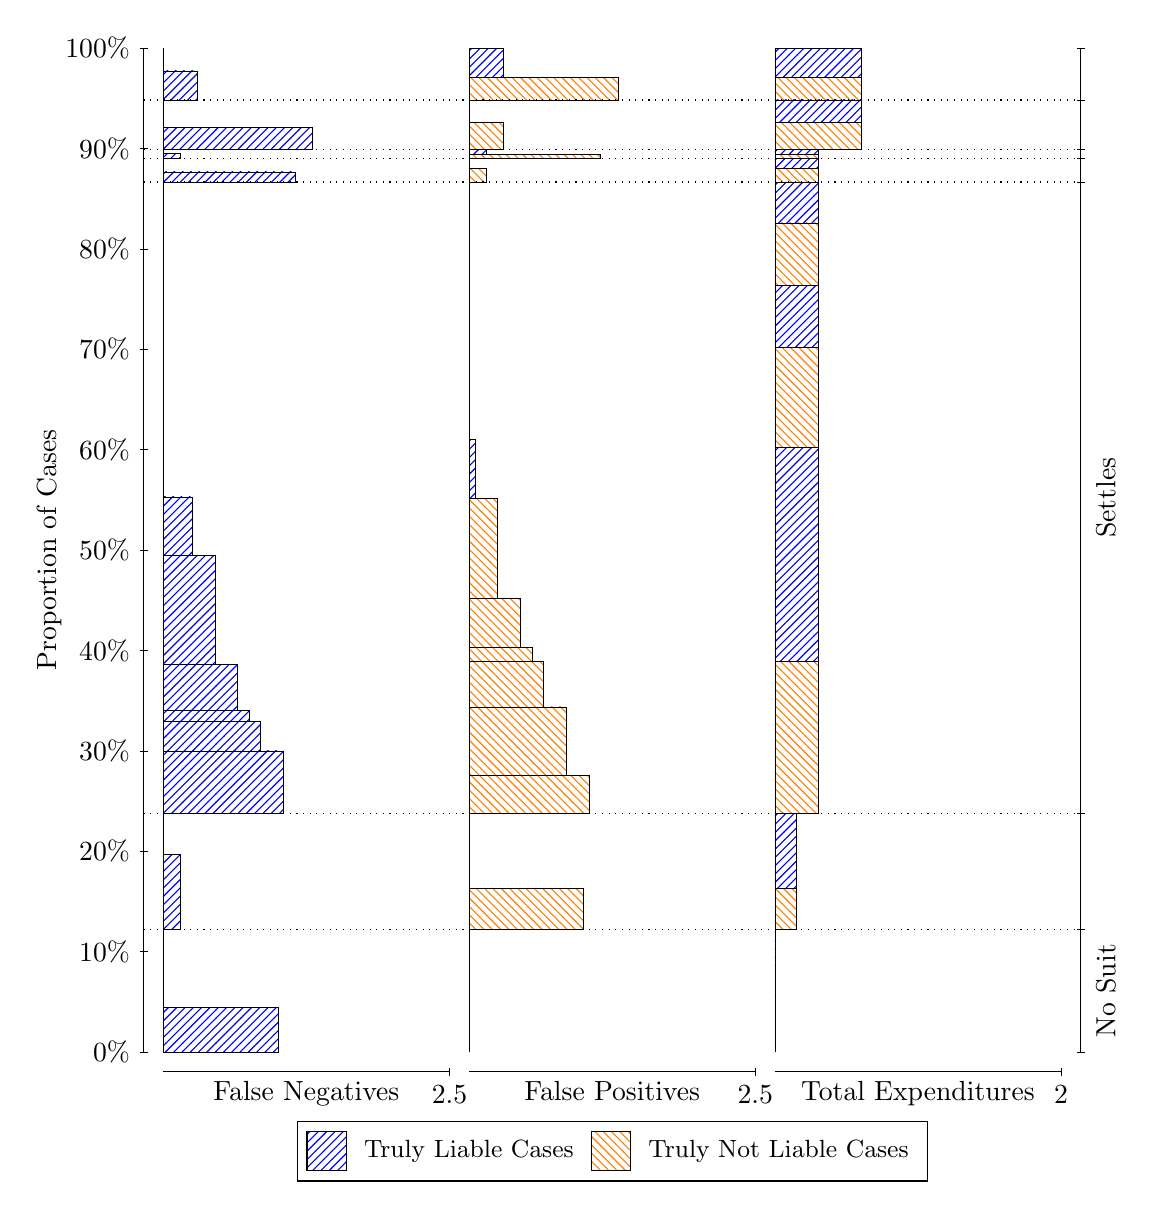
\begin{tikzpicture}
\draw[black, very thin] (1.5,1.75) -- (1.5,14.5);
\node[rotate=90, text=black, anchor=center] at (0.3, 8.125) {Proportion of Cases};
\draw[black, very thin] (1.45,1.75) -- (1.55,1.75);
\node[text=black, anchor=east] at (1.45, 1.75) {0\%};
\draw[black, very thin] (1.45,3.025) -- (1.55,3.025);
\node[text=black, anchor=east] at (1.45, 3.025) {10\%};
\draw[black, very thin] (1.45,4.3) -- (1.55,4.3);
\node[text=black, anchor=east] at (1.45, 4.3) {20\%};
\draw[black, very thin] (1.45,5.575) -- (1.55,5.575);
\node[text=black, anchor=east] at (1.45, 5.575) {30\%};
\draw[black, very thin] (1.45,6.85) -- (1.55,6.85);
\node[text=black, anchor=east] at (1.45, 6.85) {40\%};
\draw[black, very thin] (1.45,8.125) -- (1.55,8.125);
\node[text=black, anchor=east] at (1.45, 8.125) {50\%};
\draw[black, very thin] (1.45,9.4) -- (1.55,9.4);
\node[text=black, anchor=east] at (1.45, 9.4) {60\%};
\draw[black, very thin] (1.45,10.675) -- (1.55,10.675);
\node[text=black, anchor=east] at (1.45, 10.675) {70\%};
\draw[black, very thin] (1.45,11.95) -- (1.55,11.95);
\node[text=black, anchor=east] at (1.45, 11.95) {80\%};
\draw[black, very thin] (1.45,13.225) -- (1.55,13.225);
\node[text=black, anchor=east] at (1.45, 13.225) {90\%};
\draw[black, very thin] (1.45,14.5) -- (1.55,14.5);
\node[text=black, anchor=east] at (1.45, 14.5) {100\%};

\draw[black, very thin] (13.4,1.75) -- (13.4,14.5);
\draw[black, very thin] (13.35,1.75) -- (13.45,1.75);
\node[anchor=west] at (13.35, 1.75) {};
\draw[black, very thin] (13.35,3.3063) -- (13.45,3.3063);
\node[anchor=west] at (13.35, 3.3063) {};
\draw[black, very thin] (13.35,4.7802) -- (13.45,4.7802);
\node[anchor=west] at (13.35, 4.7802) {};
\draw[black, very thin] (13.35,12.798) -- (13.45,12.798);
\node[anchor=west] at (13.35, 12.798) {};
\draw[black, very thin] (13.35,13.098) -- (13.45,13.098);
\node[anchor=west] at (13.35, 13.098) {};
\draw[black, very thin] (13.35,13.212) -- (13.45,13.212);
\node[anchor=west] at (13.35, 13.212) {};
\draw[black, very thin] (13.35,13.84) -- (13.45,13.84);
\node[anchor=west] at (13.35, 13.84) {};
\draw[black, very thin] (13.35,14.5) -- (13.45,14.5);
\node[anchor=west] at (13.35, 14.5) {};

\draw[black, very thin, pattern color=blue, pattern=north east lines] (1.75,1.75) rectangle (3.2033,2.3149);
\draw[black, very thin, pattern color=orange, pattern=north west lines] (1.75,2.3149) rectangle (1.75,3.3063);
\draw[black, very thin, pattern color=blue, pattern=north east lines] (1.75,3.3063) rectangle (1.968,4.2545);
\draw[black, very thin, pattern color=orange, pattern=north west lines] (1.75,4.2545) rectangle (1.75,4.7802);
\draw[black, very thin, pattern color=blue, pattern=north east lines] (1.75,4.7802) rectangle (3.276,5.5725);
\draw[black, very thin, pattern color=blue, pattern=north east lines] (1.75,5.5725) rectangle (2.9853,5.9507);
\draw[black, very thin, pattern color=blue, pattern=north east lines] (1.75,5.9507) rectangle (2.84,6.09);
\draw[black, very thin, pattern color=blue, pattern=north east lines] (1.75,6.09) rectangle (2.6947,6.677);
\draw[black, very thin, pattern color=blue, pattern=north east lines] (1.75,6.677) rectangle (2.404,8.0525);
\draw[black, very thin, pattern color=blue, pattern=north east lines] (1.75,8.0525) rectangle (2.1133,8.8);
\draw[black, very thin, pattern color=orange, pattern=north west lines] (1.75,8.8) rectangle (1.75,12.798);
\draw[black, very thin, pattern color=blue, pattern=north east lines] (1.75,12.798) rectangle (3.4213,12.926);
\draw[black, very thin, pattern color=orange, pattern=north west lines] (1.75,12.926) rectangle (1.75,13.098);
\draw[black, very thin, pattern color=blue, pattern=north east lines] (1.75,13.098) rectangle (1.968,13.163);
\draw[black, very thin, pattern color=orange, pattern=north west lines] (1.75,13.163) rectangle (1.75,13.212);
\draw[black, very thin, pattern color=blue, pattern=north east lines] (1.75,13.212) rectangle (3.6393,13.493);
\draw[black, very thin, pattern color=orange, pattern=north west lines] (1.75,13.493) rectangle (1.75,13.84);
\draw[black, very thin, pattern color=blue, pattern=north east lines] (1.75,13.84) rectangle (2.186,14.209);
\draw[black, very thin, pattern color=orange, pattern=north west lines] (1.75,14.209) rectangle (1.75,14.5);
\draw[black, very thin, pattern color=orange, pattern=north west lines] (5.6333,1.75) rectangle (5.6333,2.7414);
\draw[black, very thin, pattern color=blue, pattern=north east lines] (5.6333,2.7414) rectangle (5.6333,3.3063);
\draw[black, very thin, pattern color=orange, pattern=north west lines] (5.6333,3.3063) rectangle (7.0867,3.832);
\draw[black, very thin, pattern color=blue, pattern=north east lines] (5.6333,3.832) rectangle (5.6333,4.7802);
\draw[black, very thin, pattern color=orange, pattern=north west lines] (5.6333,4.7802) rectangle (7.1593,5.2608);
\draw[black, very thin, pattern color=orange, pattern=north west lines] (5.6333,5.2608) rectangle (6.8687,6.1315);
\draw[black, very thin, pattern color=orange, pattern=north west lines] (5.6333,6.1315) rectangle (6.578,6.7146);
\draw[black, very thin, pattern color=orange, pattern=north west lines] (5.6333,6.7146) rectangle (6.4327,6.8848);
\draw[black, very thin, pattern color=orange, pattern=north west lines] (5.6333,6.8848) rectangle (6.2873,7.5065);
\draw[black, very thin, pattern color=orange, pattern=north west lines] (5.6333,7.5065) rectangle (5.9967,8.7781);
\draw[black, very thin, pattern color=blue, pattern=north east lines] (5.6333,8.7781) rectangle (5.706,9.5256);
\draw[black, very thin, pattern color=blue, pattern=north east lines] (5.6333,9.5256) rectangle (5.6333,12.798);
\draw[black, very thin, pattern color=orange, pattern=north west lines] (5.6333,12.798) rectangle (5.8513,12.97);
\draw[black, very thin, pattern color=blue, pattern=north east lines] (5.6333,12.97) rectangle (5.6333,13.098);
\draw[black, very thin, pattern color=orange, pattern=north west lines] (5.6333,13.098) rectangle (7.3047,13.147);
\draw[black, very thin, pattern color=blue, pattern=north east lines] (5.6333,13.147) rectangle (5.8513,13.212);
\draw[black, very thin, pattern color=orange, pattern=north west lines] (5.6333,13.212) rectangle (6.0693,13.559);
\draw[black, very thin, pattern color=blue, pattern=north east lines] (5.6333,13.559) rectangle (5.6333,13.84);
\draw[black, very thin, pattern color=orange, pattern=north west lines] (5.6333,13.84) rectangle (7.5227,14.131);
\draw[black, very thin, pattern color=blue, pattern=north east lines] (5.6333,14.131) rectangle (6.0693,14.5);
\draw[black, very thin, pattern color=orange, pattern=north west lines] (9.5167,1.75) rectangle (9.5167,2.7414);
\draw[black, very thin, pattern color=blue, pattern=north east lines] (9.5167,2.7414) rectangle (9.5167,3.3063);
\draw[black, very thin, pattern color=orange, pattern=north west lines] (9.5167,3.3063) rectangle (9.7892,3.832);
\draw[black, very thin, pattern color=blue, pattern=north east lines] (9.5167,3.832) rectangle (9.7892,4.7802);
\draw[black, very thin, pattern color=orange, pattern=north west lines] (9.5167,4.7802) rectangle (10.062,6.7146);
\draw[black, very thin, pattern color=blue, pattern=north east lines] (9.5167,6.7146) rectangle (10.062,9.4246);
\draw[black, very thin, pattern color=orange, pattern=north west lines] (9.5167,9.4246) rectangle (10.062,10.696);
\draw[black, very thin, pattern color=blue, pattern=north east lines] (9.5167,10.696) rectangle (10.062,11.488);
\draw[black, very thin, pattern color=orange, pattern=north west lines] (9.5167,11.488) rectangle (10.062,12.28);
\draw[black, very thin, pattern color=blue, pattern=north east lines] (9.5167,12.28) rectangle (10.062,12.798);
\draw[black, very thin, pattern color=orange, pattern=north west lines] (9.5167,12.798) rectangle (10.062,12.97);
\draw[black, very thin, pattern color=blue, pattern=north east lines] (9.5167,12.97) rectangle (10.062,13.098);
\draw[black, very thin, pattern color=orange, pattern=north west lines] (9.5167,13.098) rectangle (10.062,13.147);
\draw[black, very thin, pattern color=blue, pattern=north east lines] (9.5167,13.147) rectangle (10.062,13.212);
\draw[black, very thin, pattern color=orange, pattern=north west lines] (9.5167,13.212) rectangle (10.607,13.559);
\draw[black, very thin, pattern color=blue, pattern=north east lines] (9.5167,13.559) rectangle (10.607,13.84);
\draw[black, very thin, pattern color=orange, pattern=north west lines] (9.5167,13.84) rectangle (10.607,14.131);
\draw[black, very thin, pattern color=blue, pattern=north east lines] (9.5167,14.131) rectangle (10.607,14.5);
\draw[black, dotted] (1.5,3.3063) -- (13.4,3.3063);
\draw[black, dotted] (1.5,4.7802) -- (13.4,4.7802);
\draw[black, dotted] (1.5,12.798) -- (13.4,12.798);
\draw[black, dotted] (1.5,13.098) -- (13.4,13.098);
\draw[black, dotted] (1.5,13.212) -- (13.4,13.212);
\draw[black, dotted] (1.5,13.84) -- (13.4,13.84);
\draw[black, very thin] (1.75,1.5) -- (5.3833,1.5);
\node[text=black, anchor=north] at (3.5667, 1.5) {False Negatives};
\draw[black, very thin] (5.3833,1.45) -- (5.3833,1.55);
\node[text=black, anchor=north] at (5.3833, 1.45) {2.5};

\draw[black, very thin] (5.6333,1.5) -- (9.2667,1.5);
\node[text=black, anchor=north] at (7.45, 1.5) {False Positives};
\draw[black, very thin] (9.2667,1.45) -- (9.2667,1.55);
\node[text=black, anchor=north] at (9.2667, 1.45) {2.5};

\draw[black, very thin] (9.5167,1.5) -- (13.15,1.5);
\node[text=black, anchor=north] at (11.333, 1.5) {Total Expenditures};
\draw[black, very thin] (13.15,1.45) -- (13.15,1.55);
\node[text=black, anchor=north] at (13.15, 1.45) {2};

\node[text=black, centered, rotate=90] at (13.72, 2.5281) {No Suit};

\node[text=black, centered, rotate=90] at (13.72, 8.789) {Settles};





\draw (7.449999999999999,1.5) node[draw=none] (baseCoordinate) {};
\begin{scope}[align=center]
        \matrix[scale=0.5, draw=black, below=0.5cm of baseCoordinate, nodes={draw}, column sep=0.1cm]{
            \node[rectangle, draw, minimum width=0.5cm, minimum height=0.5cm, pattern color=blue, pattern=north east lines] {}; &
            \node[draw=none, font=\small, text=black] (B) {Truly Liable Cases}; &
            \node[rectangle, draw, minimum width=0.5cm, minimum height=0.5cm, pattern color=orange, pattern=north west lines] {}; &
            \node[draw=none, font=\small, text=black] (B) {Truly Not Liable Cases}; \\
            };
\end{scope}

\end{tikzpicture}
\end{document}